\section{Anàlisi i visualització de les dades}\label{sec:data-analysis}

\begin{frame}{Metodologia}
    \begin{itemize}
        \item Tipologia:
        \begin{itemize}
            \item S’ha complert aquest criteri en algun moment.
            \item Per quin període temporal es compleix el criteri X, Y i Z.
            \item Donat aquest conjunt de dades vull extraure aquesta informació per aquest període de temps.
        \end{itemize}
        \item Extraurem la informació de les nostres bases de dades.
        \item Amb l’ajuda de \textit{Grafana} representarem de forma visual el nostre cas d’ús i les conclusions extretes d’aquest.
        \item L'anàlisi pot ser directament sobre \textit{Grafana} si el volum de dades ho permet.
    \end{itemize}
\end{frame}

\begin{frame}{Casos d'ús d'exemple}
    \begin{itemize}
        \item Recurs més accedit durant un període de temps.
        \item Accessos amb el seu contingut alterat.
        \item Condicions d'accés dels accessos a recursos de l'EPSEVG.
    \end{itemize}
\end{frame}

%\begin{frame}{Recurs més accedit durant un període de temps I}
%    \begin{itemize}
%        \item Donat un període de temps, volem saber quin, o quins recursos són els més accedits.
%        \item També volem esbrinar com ha sigut la seva evolució al llarg del temps.
%        \item Quins paràmetres caracteritzen aquests accessos, vora quines hores es produeixen, mitjançant quins mètodes d'HTTP, quin és el codi de resposta més habitual\dots i molts més atributs.
%    \end{itemize}
%\end{frame}
%
%\begin{frame}{Recurs més accedit durant un període de temps II}
%    \begin{center}
%        \texttt{2099.1/18556} \\
%        ``Diseño de una aplicación Android para calcular el potencial de generación de energía eléctrica fotovoltaica.''
%    \end{center}
%    \begin{figure}
%        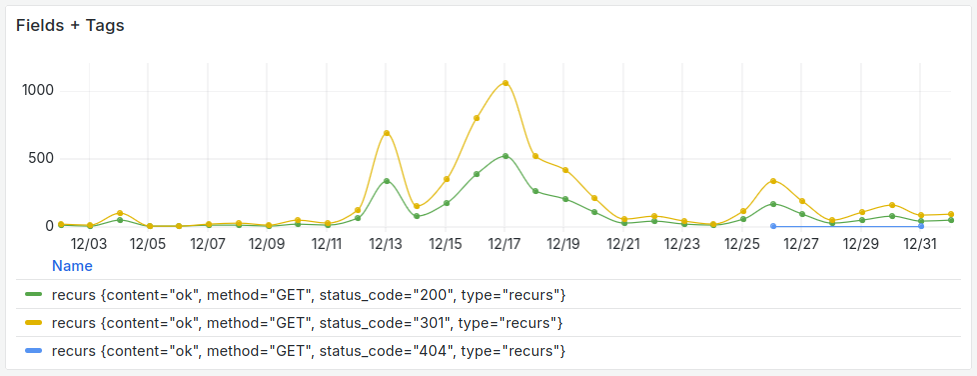
\includegraphics[width=\textwidth]{figures/most-accessed-resource}
%        \label{fig:use-case-1}
%    \end{figure}
%\end{frame}
%
%\begin{frame}{Accessos amb el seu contingut alterat I}
%    \begin{itemize}
%        \item Donat un espai de temps, volem consultar quants accessos s'han produït amb malformacions al seu contingut.
%
%        \begin{itemize}
%            \item Les malformacions del contingut del accessos corresponen a registres que difereixen molt respecte el format general.
%            \item Durant l'etapa d'anàlisi i emmagatzematge dels logs, vam marcar aquells sospitosos amb una etiqueta.
%        \end{itemize}
%
%        \item També volem esbrinar com ha sigut la seva evolució al llarg del temps, a més dels paràmetres que s'utilitzen.
%    \end{itemize}
%\end{frame}
%
%\begin{frame}{Accessos amb el seu contingut alterat II}
%    \begin{figure}
%        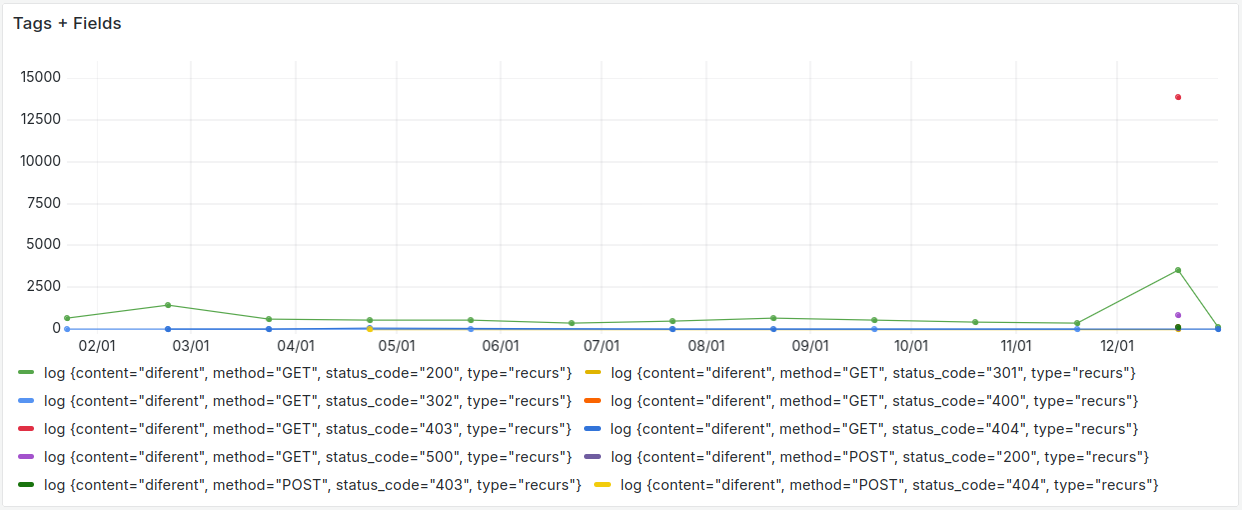
\includegraphics[width=\textwidth]{figures/possible-attacks}
%        \label{fig:use-case-2}
%
%    \end{figure}
%\end{frame}
%
%\begin{frame}{Accessos amb el seu contingut alterat III}
%    \begin{figure}
%        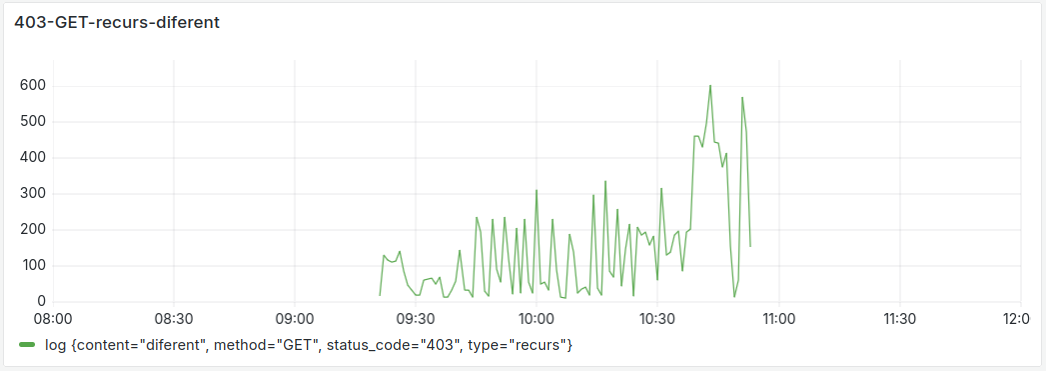
\includegraphics[width=\textwidth]{figures/possible-attacks-403}
%        \label{fig:use-case-2-1}
%    \end{figure}
%    \begin{figure}
%        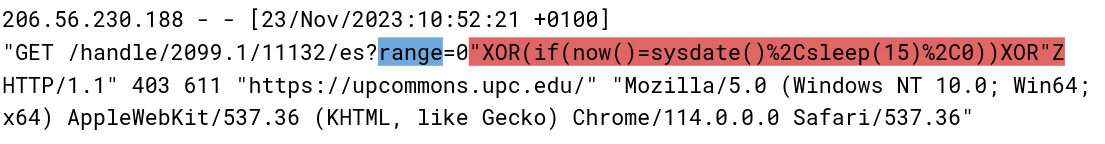
\includegraphics[width=\textwidth]{figures/log-attack}
%        \label{fig:use-case-2-2}
%    \end{figure}
%\end{frame}
%
%\begin{frame}{Condicions d'accés dels accessos a recursos de l'EPSEVG I}
%    \begin{itemize}
%        \item Donat un període de temps, volem saber quines són les condicions d'accés dels recursos de l'EPSEVG consultats.
%        \item Volem analitzar dels registres aquells que siguin accessos a recursos de l'EPSEVG, i determinar si aquests són d'accés obert, restringits per l'usuari, per acord de confidencialitat, restringit a la comunitat universitària, etcètera.
%    \end{itemize}
%\end{frame}
%
%\begin{frame}{Condicions d'accés dels accessos a recursos de l'EPSEVG II}
%    \begin{figure}
%        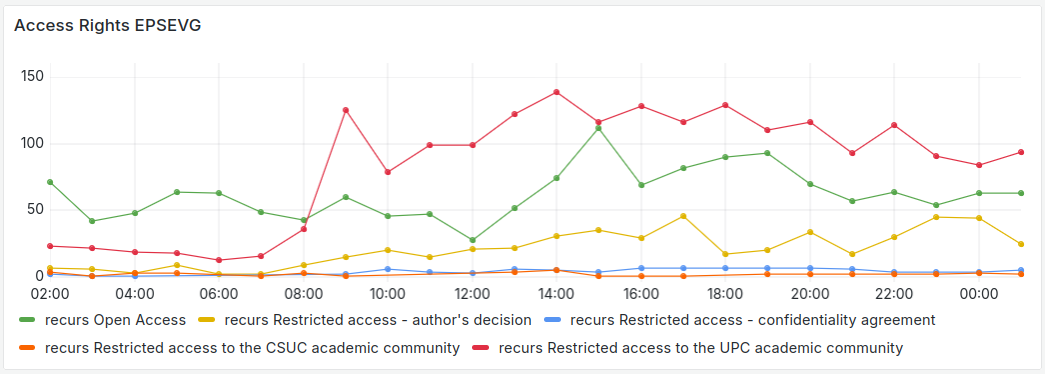
\includegraphics[width=\textwidth]{figures/access-rights-epsevg}
%        \label{fig:use-case-3}
%    \end{figure}
%\end{frame}